\usetikzlibrary{calc}
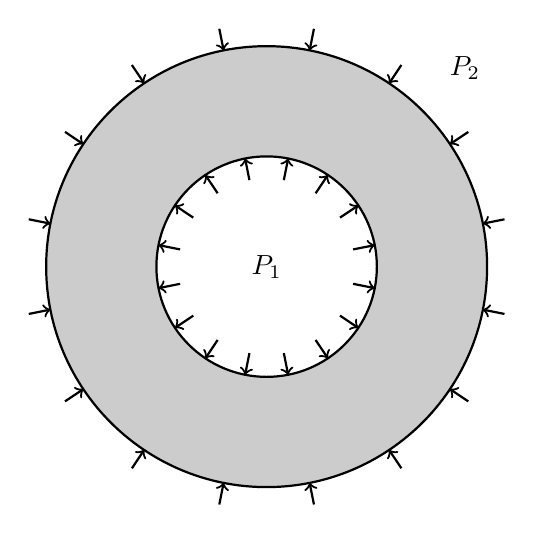
\begin{tikzpicture}[thick, scale = 0.14]
\filldraw[fill=gray!40!white, draw=black] (0, 0) circle (20cm);
\filldraw[fill=white, draw=black] (0, 0) circle (10cm);

\foreach \x in {0,...,3}{
	\draw[->] ($8*({cos(22.5*\x + 11.25)}, {sin(22.5*\x + 11.25)})$) -- ($10*({cos(22.5*\x + 11.25)}, {sin(22.5*\x + 11.25)})$);
	\draw[->] ($8*({cos(22.5*\x + 11.25)}, {-sin(22.5*\x + 11.25)})$) -- ($10*({cos(22.5*\x + 11.25)}, {-sin(22.5*\x + 11.25)})$);
	\draw[->] ($8*({-cos(22.5*\x + 11.25)}, {sin(22.5*\x + 11.25)})$) -- ($10*({-cos(22.5*\x + 11.25)}, {sin(22.5*\x + 11.25)})$);
	\draw[->] ($8*({-cos(22.5*\x + 11.25)}, {-sin(22.5*\x + 11.25)})$) -- ($10*({-cos(22.5*\x + 11.25)}, {-sin(22.5*\x + 11.25)})$);

	\draw[->] ($22*({cos(22.5*\x + 11.25)}, {sin(22.5*\x + 11.25)})$) -- ($20*({cos(22.5*\x + 11.25)}, {sin(22.5*\x + 11.25)})$);
	\draw[->] ($22*({cos(22.5*\x + 11.25)}, {-sin(22.5*\x + 11.25)})$) -- ($20*({cos(22.5*\x + 11.25)}, {-sin(22.5*\x + 11.25)})$);
	\draw[->] ($22*({-cos(22.5*\x + 11.25)}, {sin(22.5*\x + 11.25)})$) -- ($20*({-cos(22.5*\x + 11.25)}, {sin(22.5*\x + 11.25)})$);
	\draw[->] ($22*({-cos(22.5*\x + 11.25)}, {-sin(22.5*\x + 11.25)})$) -- ($20*({-cos(22.5*\x + 11.25)}, {-sin(22.5*\x + 11.25)})$);}
	\node at (0, 0) (c) {$P_1$};
    \node at (18, 18) (c) {$P_2$};    

\end{tikzpicture}